On souhaite comparer les résultats de convergence de réseaux entraînés sur MNIST avec ceux entraînés sur FashionMNIST pour les mêmes expériences, dans le but d'en tirer des caractéristiques et une différence globale de comportement des réseaux liés à ces deux jeux de données. Prenons par exemple le réseau $\mathcal{S}$MorphNetTanh composé de deux couches morphologiques, et que l'on munit simplement d'un partage de poids doux (contrainte entre $w_1$ et $w_2$ dans la \textit{loss}, eq. \ref{MSEpConstraintFilters}). On fait alors une analyse rapide en constatant uniquement la forme des noyaux du réseau dans son état final, moyennée sur 6 runs par expérience. On obtient les résultats représentés sur la figure \ref{fig:results_mnist_vs_fashionmnist}, avec MNIST à gauche (\ref{fig:suk1}) et FashionMNIST à droite (\ref{fig:suk2}). \\

%figure
\vspace{0.2mm}
\begin{figure}[ht]
  \begin{center}
      \subfigure[Avec MNIST]{
          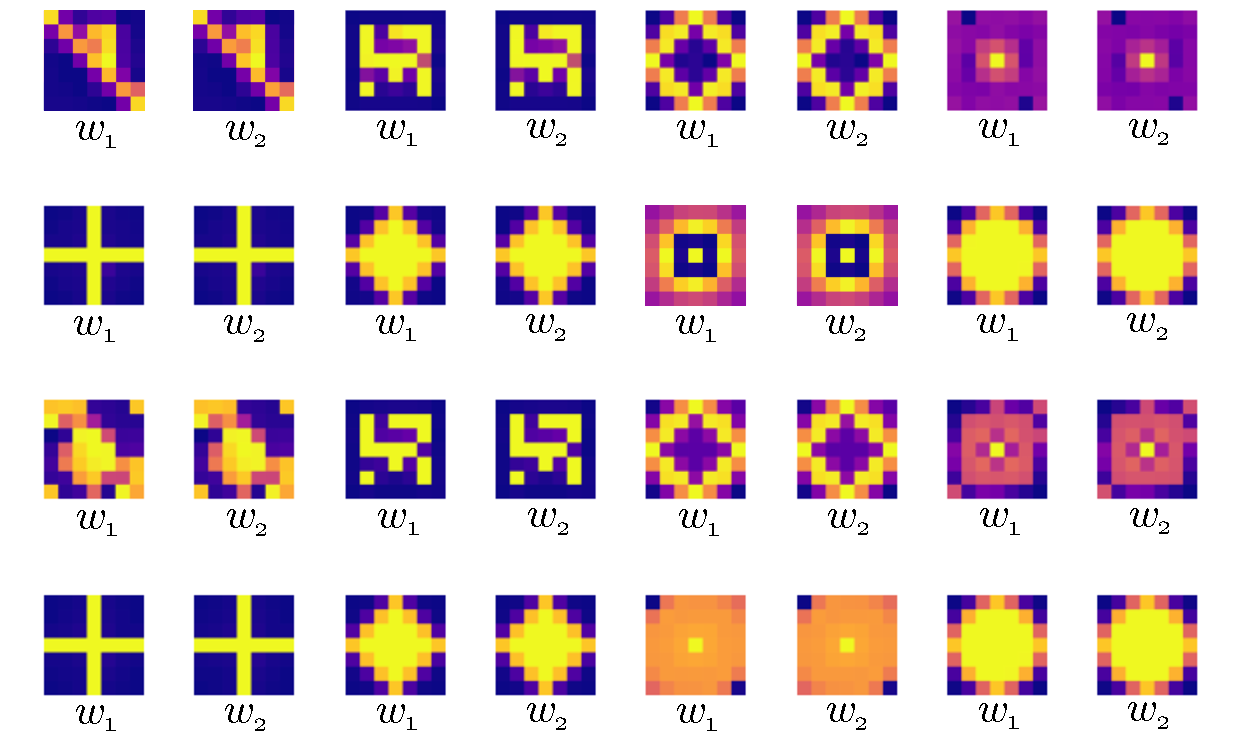
\includegraphics[width=0.47\textwidth]{parts/4-analyse_des_reseaux/impact_database/figures/ft1.pdf}
          \label{fig:suk1}}
      \hspace{1.6mm}
      \subfigure[Avec FashionMNIST]{
          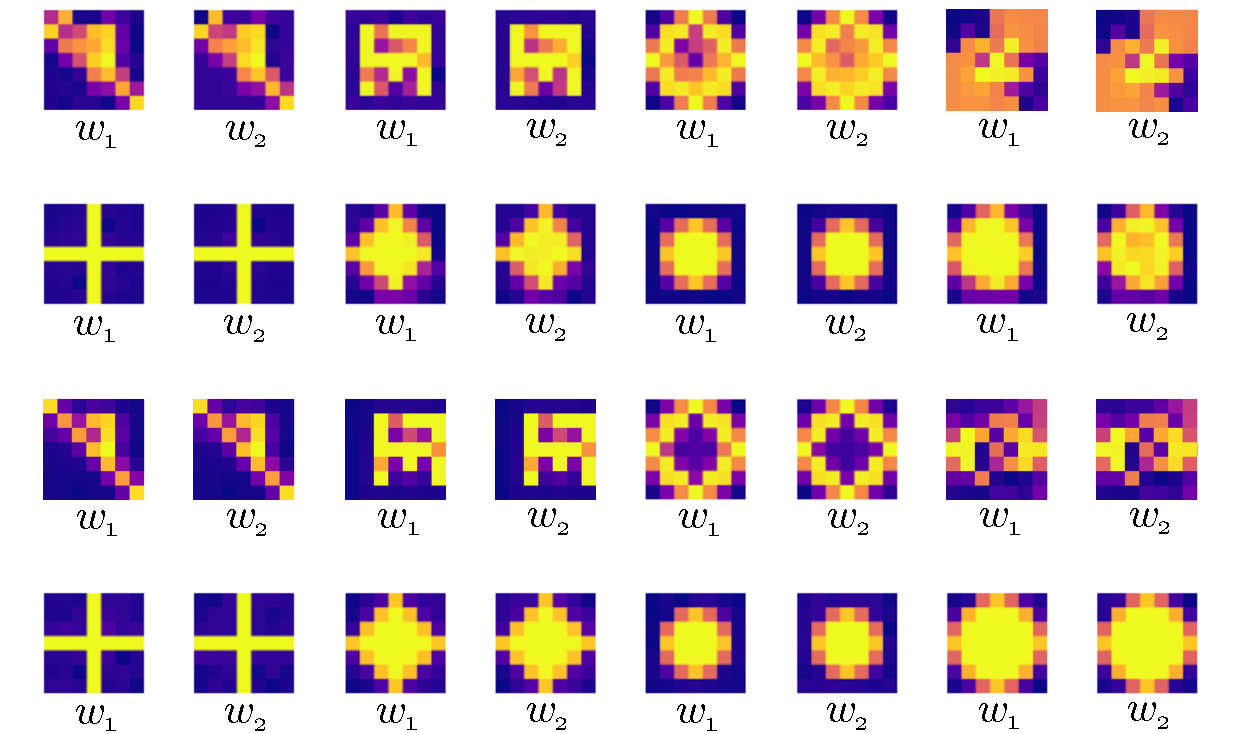
\includegraphics[width=0.47\linewidth]{parts/4-analyse_des_reseaux/impact_database/figures/ft2.pdf}
          \label{fig:suk2}}
    \caption{ \centering Noyaux $w$ associés par paires du réseau $\mathcal{S}$MorphNetTanh après convergence, entraîné sur les jeux de données MNIST (\ref{fig:suk1}) et FashionMNIST (\ref{fig:suk2}). Les cases à gauche et à droite de même emplacement correspondent à la même expérience.}
    \label{fig:results_mnist_vs_fashionmnist}
  \end{center}
\end{figure}

\vspace{-2.4mm}
Les différences de résultats des noyaux $w$ pour ces expériences-là entre les deux jeux MNIST et FashionMNIST sont très notables. Certains résultats semblent meilleurs avec la banque FashionMNIST, comme ceux avec les structures cibles \textit{adiag} pour l'ouverture (troisième ligne [milieu bas] première paire [tout à gauche]) ou \textit{disk2} (deuxième ligne troisième paire, et dernière ligne troisième paire), tandis que d'autres semblent meilleurs avec FashionMNIST, comme ceux avec les structures cibles \textit{brand} (première ligne deuxième paire, et troisième ligne deuxième paire) ou \textit{complex} pour la fermeture (première ligne troisième paire). Les résultats sont très diversifiés, et ne plaident pas significativement en la faveur d'un des deux jeux de données. \\

\vspace{-1.0mm}
\noindent Les mêmes observations et la même conclusion peuvent être faites avec les autres réseaux morphologiques ($p$ConvNet, $\mathcal{L}$MorphNet et $\mathcal{S}$MorphNet) et dans les autres configurations de réseaux (avec/sans partage de poids, avec/sans contrainte géométrique sur $w$ ou sur $\alpha / p$, initialisation aléatoire / initialisation gaussienne, etc.).


\newpage

Plusieurs hypothèses peuvent expliquer ces différences de résultats entre les deux jeux de données. 
En particulier, l'aspect << fin >> des objets sur les images MNIST doit impacter l'entraînement des réseaux de manière différente que ne le font les aspects << épais >> et << étendu >> des objets sur les images FashionMNIST.
Les objets fins sur les images peuvent par exemple s'effacer intégralement avec une petite opération d'\textit{érosion}, et donc la prédiction sur l'érosion serait moins facile à faire pour les réseaux morphologiques ciblant cette opération ou bien ciblant l'ouverture (qui commence par une érosion, et donc peut directement effacer les objets avant même la dilatation). \\

\vspace{-1.6mm}
\noindent C'est en effet ce que l'on observe sur la figure \ref{fig:results_mnist_vs_fashionmnist} : on constate avec MNIST (\ref{fig:suk1}) que ce sont les résultats sur la fermeture (moitié supérieure) qui semblent plus précis que ceux sur l'ouverture (moitié inférieure), notamment en observant les structures \textit{adiag} et \textit{complex}. Avec FashionMNIST (\ref{fig:suk2}), on constate l'inverse : ce sont les résultats sur l'ouverture (dessous) qui semblent plus précis que ceux sur la fermeture (dessus). Cela peut s'expliquer par la trop petite place laissée au fond de l'image sur son support, à cause de l'épaisseur des objets, et donc par le fait qu'une dilatation (et donc une fermeture) supprimerait une trop grande partie du fond, ce qui rendrait les prédictions sur la dilatation et la fermeture avec FashionMNIST plus délicates.

\vspace{1.0mm}

%%%

%-> Les différences sont notables (certains mieux, d'autres pires)
%-> C'est la même conclusion avec les autres réseaux et les autres configuration de réseaux (avec/sans contrainte, avec/sans partage de poids, avec/sans initialisation gaussienne, etc.)

%%%-> Dire que sur MNIST (avec images en positif), on aurait plutôt dit que c'est l'érosion qui poserait problème, car les éléments sont très fins et s'effacent quasiment intégralement avec une petite érosion, donc que la prédiction sur l'érosion serait moins facile à faire... Mais on observe l'inverse ! Warum ??? <=== !!!NON!!!, pas pour l'exemple choisi ! Par contre, avec une initialisation gaussienne par exemple, oui en effet...